%%%%%%%%%%%%%%%%%%%%%%%%%%%%%%%%%%%%%%%%%%%
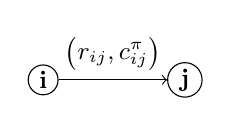
\begin{tikzpicture}[nodes={font=\bf\small}, scale=0.45]
%  \draw [help lines] (-1,-1) grid (8,5);o

\tikzstyle{tasknode}=[%
  draw,
  circle,
  minimum width=0.4,
  inner sep=0.5mm,
]

% nodes
\node [tasknode] (i) at (2, 0) {i};
\node [tasknode] (j) at (6, 0) {j};

\path [draw, ->] (i) -- node[above] {$\left(r_{ij},c_{ij}^{\pi}\right)$} (j);

\end{tikzpicture} 
%%%%%%%%%%%%%%%%%%%%%%%%%%%%%%%%%%%%%%%%%%%
